\documentclass[a4paper,12pt,landscape]{article}
\usepackage{fullpage} % for 1.5 cm margins
\renewcommand{\familydefault}{\sfdefault} % so it doesn't look like LaTeX
\usepackage{helvet}
\usepackage[british]{isodate}
\usepackage{abstract}
\renewcommand{\abstractname}{Overview}
\newcommand{\tickbox}{\framebox(12,12){} }
\newcommand{\fillbox}{\begin{tabular}{|l|}
  \hspace{60pt} \\
  \hline
\end{tabular} }
\usepackage{enumitem, amssymb} % for checklists
\newlist{todolist}{itemize}{1}
\setlist[todolist]{label=$\tickbox$, parsep=1em}
\raggedright
\raggedbottom
\usepackage{multicol}
\usepackage{graphicx}
\usepackage{parskip}
\usepackage{draftwatermark}
\SetWatermarkText{DRAFT}
\SetWatermarkScale{0.5}
\SetWatermarkLightness{0.9}


\newcommand{\documenttitle}{Shropshire Botanical Society Online Flora}
\newcommand{\documentauthor}{Joe J Collins}
\newcommand{\nbnrecords}[1]{\href{https://records-ws.nbnatlas.org/#1}{\detokenize{https://records-ws.nbnatlas.org/#1}}}
\newcommand{\wireframe}[1]{\includegraphics[width=0.85\textwidth,height=\textheight,keepaspectratio]{#1}\clearpage}

\title{Shropshire Botanical Society Online Flora\\
Draft Specification}
\author{\documentauthor}
\date{\today}

\usepackage[pdftex,
  pdftitle={\documenttitle}, 
  pdfauthor={\documentauthor},
  pdfsubject={\documenttitle}]{hyperref}

\begin{document}
\maketitle
\begin{abstract}
  \begin{center}
    \begin{minipage}{0.5\textwidth}
      \strut\\
      The Shropshire Botanical Society is seeking
      to renew it's Online Flora web application.
      This specification out lines the hoped for functionality
      together with the technical
      and
      development constraints of the work.
    \end{minipage}
  \end{center}
\end{abstract}

\newpage% Blank page behind title page
\mbox{}
\clearpage

\begin{multicols*}{2}
  \setcounter{tocdepth}{3}
  \tableofcontents
  \vfill\strut
  \columnbreak

  \section{Background}
  The Shropshire Botanical Society
  has been dedicated to promoting the enjoyment,
  understanding and conservation of the flora of Shropshire
  since the 18\textsuperscript{th} century.
  One of the principle activities of the Society is to collect and maintain records 
  of plant sightings within the historical boundaries of the county of Shropshire.
  Since 2003 the Society has made these records freely available online via a bespoke web application
  or Online Flora.
  This original Online Flora was written using
  PHP and the CodeIgniter Web Framework
  backed by a MySql database.
  The web application is still available at 
  \href{https://captain-blue.azurewebsites.net/}{captain-blue.azurewebsites.net}
  but unfortunately the data is now many years out of date.

  Maintaining and updating the database has proved to be challenging.
  Additionally the application was conceived prior to the introduction of the iPhone
  and it not suited to mobile use.
  Hence the Society seeks to renew the web application,
  to provide a more modern mobile interface
  and to use up to date data stored
  by the \href{https://nbnatlas.org/}{National Biodiversity Network Atlas}.
  Currently all the Society's records are submitted to the 
  National Biodiversity Network Atlas
  and since 2017 the Society's records have been available via a web service at
  the \href{https://api.nbnatlas.org/}{NBN Web service API}.
  Using the NBN Web service API provides reliable data source
  and
  a supported service for maintaining and updating the Society's records.

  \clearpage

  \section{Objective}
  To replicate the functionality of the original Online Flora
  in a responsive mobile design
  using data sourced from the NBN Web service API.

  The Online Flora is to be used for searching the Society's records
  but not for entering new records.
  Maintaining and updating the data is conducted via a separate manual process.
  Searches of the database are conducted for three different geographical scenarios.

  \section{Context}

  \subsection{Users and Usage}
  Users of the Online Flora are typically
  members of the Society
  and
  as such are often very experienced botanists.
  In a typical scenario a member of the Society
  (intending to visit a location)
  would search for a list of species that have previously
  been sighted at a location.
  It is the community or suite of species at a location that is of most interest.
  For an experienced botanist a species list for a location
  can provide information about
  the ecology, geology and history of a location,
  but will also indicate what other species might be present but have not yet been observed.
  Ideally the member of the Society
  would also wish to drill down to see individual records of species sightings,
  with dates, attributions and further details.
  This background will give a botanist
  some insight about how much weight or credence can be given to individual sightings.

  The Online Flora will serve three scenarios for
  searching for species lists.

  \begin{description}
      \item[Search Shropshire:]
        searching all the records of based on the name of the plant.
        Allowing the user to drill down to a single sighting record
        or
        showing a map of grid squares with records for a named plant.
      \item[Search by Site:]
        searching for a named site,
        then listing the names of plants for that named site.
        Again allowing the user to drill down to a single sighting record.
      \item[Search by Monad or Grid Square:]
        Selecting a 1 km grid square within the county of Shropshire,
        then listing the names of plants for that named site.
        Again allowing the user to drill down to a single sighting record.
  \end{description}

  These three scenarios are shown in the diagram below.
  \clearpage

  \wireframe{./wireframes/Overview.png}%

  \subsection{Categories of Plants}
  Gaining experience identifying plants is a lifetimes work
  and members of the Society will often
  focus their attention on one category of plants.
  So the Society's observation records
  are separated into \textbf{vascular plants} and \textbf{bryophytes},
  (two categories within the kingdom of all plants).
  A member of the Society will often wish to limit their searches to the
  category of plants they are most interested in.

  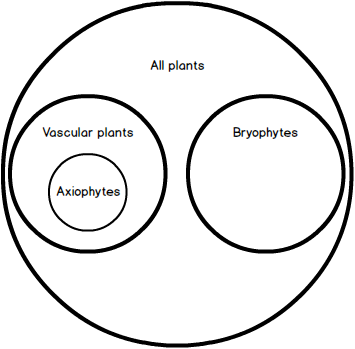
\includegraphics[width=0.4\textwidth,height=\textheight,keepaspectratio]{./wireframes/Categories.png}

  For the vascular plants
  the concept of indicator species is highlighted
  by a sub group of vascular plants
  (referred to as \textbf{axiophytes})
  These are plants that are archetypical or axiomatic for a particular ecological environment.
  So a member of the Society interested in vascular plants
  will often wish to see only the axiophytes
  to gain a better understanding of the ecological environment
  at a particular site.

  \subsection{Data Storage}
  The National Biodiversity Network Atlas (NBN)
  provides a service to maintain and distribute biological records
  for the United kingdom.
  The Shropshire Botanical Society contributes records to the NBN
  via the \href{https://sites.google.com/view/sedn/home}{Shropshire Ecological Data Network} (SEDN).
  So all the botanical records for Shropshire
  are contained within the SEDN dataset on the NBN service
  (\href{occurrences/search?q=data_resource_uid%3Adr782}{dataset 782}).
  There is a regular(ish) process in place for passing updates to the NBN
  so new records are added every 6 months or so. 

  The NBN provides a \href{https://api.nbnatlas.org/}{specialized API}
  to query these data which is based on Apache Solr.
  A \href{http://docs.shropshirebotany.org.uk/NBN%20Atlas%20Query%20Primer.pdf}{primer for how to use the API}
  is provided by the NBN.

  \begin{todolist}
    \item To improve performance queries should be cached on the server for about 30 days.
    \item No data should be cached on the client device.
    \item Offer `Add to Home screen' on first and fifth visit.
  \end{todolist}

\end{multicols*}

%%%%%%%%%%%%%%%%%%%%%%%%%%%%%%%%%%%%%%%%%%%%%%%%%%%%%%%%%%%%%%%%%%%%%%%%%%
\begin{multicols*}{2}[%
  \section{Search the County}%
  \subsection{Species List for County}%
  \label{sec:species-list-for-county}%
]
\thispagestyle{empty}
\wireframe{./wireframes/Species__ListForCounty.png}%

\subsubsection*{`Landing'} 

\begin{todolist}
  \item Initially the search output should be empty.
  \item By default the \textbf{Scientific} name selected first,
  since botanists tend to favour identifying
  plant species via the scientific name.
  \item If \textbf{Common} is selected set a cookie to retain the user's choice of naming type.
  \item Also set a cookie for the user's choice of plant group (bryophytes or vascular plants).
\end{todolist}

\subsubsection*{Species Search}

\begin{todolist}
  \item The search is of the entire dataset for the county.
  \item The characters entered in the search box are used to search for names beginning with those letters,
    not within the names.
    \footnote{\nbnrecords{explore/group/Plants?fq=data_resource_uid:dr782+AND+taxon_name:B*}}
  \item Clicking on \textbf{List Species} or pressing return on the desktop list executes the search.
    If the search box is empty species beginning with `A' are searched for.
  \item Any characters entered in the search box are retained after the button is clicked.
  \item The search results should be listed alphabetically by scientific name or common name,
    whichever is selected.
  \item If \textbf{Common} is selected, only the species with common names will be searched and shown.
    Any species without common names should not be included in the search results.
  \item If \textbf{Axiophytes} is selected a limited static list of scientific names will be searched and shown.
    The list of axiophytes is provided as a list of scientific species names.
    This list was last updated in 2014.
  \item Changing any radio button will renew the search using the changed set of parameters,
    without pressing return or clicking on the button.
  \item If the search result list is long pages links should be provided.
  \item The download link, downloads a zipped CSV of the search results directly from the NBN.
    \footnote{\nbnrecords{occurrences/index/download?q=data_resource_uid:dr782&fq=taxon_name:A*&reasonTypeId=11&fileType=csv}}
  \item Clicking on the scientific or common species name,
    takes you to a list of records for that species in the county.
\end{todolist}

\subsection{Records for a Single Species in the County}

\wireframe{./wireframes/Records__SingleSpeciesForCounty.png}%

\subsubsection*{Records List} 

\begin{todolist}
  \item Title is the scientific name or common name depending on which was clicked on in the previous page.
  \item The `$<<$' goes back to the search for a species name using the same search parameters.
  \item The records are sorted by date, with most recent first.
  \footnote{\nbnrecords{occurrences/search?q=data_resource_uid:dr782&fq=taxon_name:Abies\%20alba&sort=taxon_name&fsort=index&pageSize=9}}
  \item If the records list is long pages links should be provided.
  \item The download link, downloads a zipped CSV of the search results directly from the NBN.
  \item Site link goes to a list of records for the same species at the selected site.
  \item Square link goes to a list of records for the same species at the selected square.
\end{todolist}

\subsubsection*{Map} 

\begin{todolist}
  \item Zoomable but not clickable.
  \item The records are in a hidden tab on mobile devices.
  \item Showing location of the site with a pin, since we don't have shape files for the sites,
   use the location of the first record.
  \item The map overlay comes from the NBN Web Mapping Service showing a distribution map of the species.
  \item Include an outline of the county.
\end{todolist}

\clearpage
\subsection{A Single Record}

\wireframe{./wireframes/Records__SingleRecord.png}%

\subsubsection*{Record Detail} 

\begin{todolist}
  \item Title is the scientific name or common name depending on the previous page.
  \item The `$<<$' goes back to the records list for that species in the county.
  \item Show as much detail for the records as possible.
  \footnote{\nbnrecords{occurrence/4276e1be-b7d2-46b0-a33d-6fa82e97636a}}
  \item Site link goes to a list of records for the same species at the selected site.
  \item Square link goes to a list of records for the same species at the selected square.
  \item The download link, downloads a zipped CSV of the search results directly from the NBN.
\end{todolist}

\subsubsection*{Map} 

\begin{todolist}
  \item Zoomable but not clickable.
  \item In a hidden tab on mobile devices.
  \item The location of the record is marked with a square indicating the resolution of the grid reference.
\end{todolist}

\end{multicols*}

%%%%%%%%%%%%%%%%%%%%%%%%%%%%%%%%%%%%%%%%%%%%%%%%%%%%%%%%%%%%%%%%%%%%%%%%%%
\begin{multicols*}{2}[%
  \section{Search in a Site}%
  \subsection{Site List for the County}%
]
\thispagestyle{empty}
\wireframe{./wireframes/Sites__ListForCounty.png}%

\subsubsection*{Sites Search}

\begin{todolist}
  \item Initially the search output should be empty.
\end{todolist}

\subsubsection*{Sites List}

\begin{todolist}
  \item The characters entered in the search box are used to search for names beginning with those letters,
    not within the names.
    \footnote{\nbnrecords{occurrences/search?fq=location_id:[Church\%20TO\%20*]&fq=data_resource_uid:dr782&facets=location_id&facet=on&pageSize=0}}
  \item Clicking on \textbf{List Sites} or pressing return on the desktop list executes the search.
    If the search box is empty species beginning with `A' are searched for.
  \item The sites should be ordered alphabetically by the site name (i.e. the `location\_id' field from the NBN records).
  \item Any characters entered in the search box are retained after the button is clicked.
  \item Clicking on the site name take you to a species list for that site.
\end{todolist}

\clearpage

\subsection{Species List for a Site}

\wireframe{./wireframes/Species__ListForSite.png}%

\subsubsection*{Species List} 

\begin{todolist}
  \item Title is the name of the site clicked on in the previous page.
  \item The `$<<$' goes back to the previous search of site names.
  \item Changing any radio button will renew the search using the changed set of parameters.
  \item Radio button settings should be retained in a cookie.
    These values are the same as the ones used in the \hyperref[sec:species-list-for-county]{Species List for County}.

\end{todolist}

\subsubsection*{Map}

\begin{todolist}
  \item Zoomable but not clickable.
  \item In a hidden tab on mobile devices.
  \item Showing location of the site with a pin, since we don't have shape files for the sites,
   use the location of the first record of the first species.
\end{todolist}

\clearpage

\subsection{Records for a Single Species at a Site}

\wireframe{./wireframes/Records__SingleSpeciesForSite.png}%

\subsubsection*{Records List} 

\begin{todolist}
  \item Show records for that species at the selected site.
  \item Square link goes to a list of records for the same species at the selected square.
\end{todolist}

\subsubsection*{Map}

\begin{todolist}
  \item Zoomable but not clickable.
  \item In a hidden tab on mobile devices.
  \item Showing location of the site with a pin, since we don't have shape files for the sites,
   use the location of the first record.
\end{todolist}

\clearpage
\end{multicols*}

%%%%%%%%%%%%%%%%%%%%%%%%%%%%%%%%%%%%%%%%%%%%%%%%%%%%%%%%%%%%%%%%%%%%%%%%%%
\begin{multicols*}{2}[%
  \section{Search in a Square}%
  \subsection{Select a Square}%
]
\thispagestyle{empty}
\wireframe{./wireframes/Squares__Index.png}%

\subsection{Records for a Single Species at a Site}

\subsubsection*{Map Control}

\begin{todolist}
  \item Zoom in and select a 1 km grid square.
  \item A 1 km graticule to appear when the squares are big enough (for selection with a finger).
  \item Retain map zoom and centre position between visits.
  \item The `cross hair' icon to zoom to the current location using the browser Geolocation API.
\end{todolist}

\clearpage

\subsection{Species List for a Square}

\wireframe{./wireframes/Species__ListForSquare.png}%

\subsubsection*{Species List}

\begin{todolist}
  \item Title is the name of the square selected on in the previous page.
  \item The `$<<$' goes back to the map for selecting grid squares.
  \item Changing any radio button will renew the search using the changed set of parameters.
  \item Radio button settings should be retained in a cookie.
    These values are the same as the ones used in the \hyperref[sec:species-list-for-county]{Species List for County}.
\end{todolist}

\subsubsection*{Map}

\begin{todolist}
  \item Zoomable but not clickable.
  \item In a hidden tab on mobile devices.
\end{todolist}

\clearpage

\subsection{Records for a Single Species at a Site}

\wireframe{./wireframes/Records__SingleSpeciesForSquare.png}%

\subsubsection*{Records List}

\begin{todolist}
  \item Title is the name of the square and the species selected on in the previous page.
  \item The `$<<$' goes back to the species list for a grid square.
\end{todolist}

\subsubsection*{Map}

\begin{todolist}
  \item Zoomable but not clickable.
  \item In a hidden tab on mobile devices.
\end{todolist}

\clearpage
\end{multicols*}

\section{Technical Constraints}%

% Simple and convenient caching.
% Possible to source PHP developers from within the ranks of members.
% Possibility of free hosting on the Google App Engine.
% Simplest possible with the lowest barrier to entry.
% Almost any programmer should be able to work on it.

The Botanical Society has limited means
and wishes to ensure that the results of any programming effort
can be maintained and supported
into the future,
either via an open source project or via the efforts of members of the Society.
To facilitate these possibilities
the technical environment for the project is intended 
to provide a low(ish) barrier to contributions.

\begin{description}
    \item[PHP 7.3] for deployment to Google App Engine for free hosting.
    \item[CodeIgniter 4.0.4] has been used successfully in the past and provides long term file caching.
    \item[Twitter Bootstrap 4.5.2] for responsive layout.
    \item[Leaflet 1.6.0] for interactive maps.
    \item[Style Sheet] is taken from \url{https://www.shropshirebotany.org.uk/}.
      The Online Flora is to be consistent with this website,
      so should where possible reuse the same CSS classes and styles.
    \item[No database] should be used other than the NBN Web service API,
      to keep down maintenance costs.
      Any static data 
      (such as the list of axiophytes)
      should be hard coded into the application.

    \item[Commits to Github] since the Society will retain the intellectual property rights
      over any code produced.
      So all branching should be on the repository at
      at \url{https://github.com/joejcollins/captain-magenta.git}.
    \item[CI/CD] the develop branch deploys to \url{https://captain-magenta.azurewebsites.net/} on Azure
      and will be used to review progress.
\end{description}

\end{document}


